\DeclareUnicodeCharacter{2212}{-}

\documentclass[12pt,oneside,a4paper]{book} % This style for A4 format.

%Packages
\usepackage{ecproject}
\usepackage{graphicx}
\usepackage{tikz}
\usetikzlibrary{calc}
\usepackage[a4paper, margin=1in]{geometry}
\usepackage{float}
\usepackage{qrcode}
%%%Page related
\usepackage{fancyhdr} % for header & footer
\usepackage[hidelinks]{hyperref}
\usepackage[toc, nonumberlist]{glossaries} %For Glossaries - to be loaded only after hyperref package
% For code snippets
\usepackage[listings]{tcolorbox}
    \tcbuselibrary{skins,breakable}
    \tcbuselibrary{theorems}
%\ifIndentPara
\usepackage{indentfirst}
%\fi
\usepackage{setspace}
%%%Table Related
%\usepackage{booktabs}
%\usepackage{makecell}
%\usepackage{multirow}
%\usepackage{multicol}
\usepackage{booktabs}
%\usepackage{biblatex}


%Document settings
\title{Design of Vedic Multiplier using High-speed Area Efficient 3 Operands Adder  
}
%%%%%%%%%%%%%%%Minor (or) Major report%%%%%%%%%%%%%%%
%Uncomment \MinorProject line, if the report is for a Minor project.
\MinorProject
%%%%%%%%%%%%%%%%%%%%%%%%%%%%%%%%%%%%%%%%%%%%%%
%%%Student Details%%%
\stuNameA{Mohammed Ikramuddin}
\stuUSNA{1RV20LVS18}


%%%Internal Guide%%%%
\guideNameA{Dr. Govinda Raju M}
\guideDesignationA{Assistant Professor}
\guideDeptA{Dept. of ECE}
\guideOrgA{RV College of Engineering}

%%%External Guide%%%%
\guideNameB{Dr. Kariyappa B.S}
\guideDesignationB{Professor}
\guideDeptB{Dept. of ECE}
\guideOrgB{RV College of Engineering}

%\guideNameC{Dr. Ramavenkateshwaran}
%\guideDesignationC{Assistant Professor}
%\guideDeptC{Dept. of ECE}
%\guideOrgC{RV College of Engineering}

\panelMemberA{Dr. Kariyappa B.S}
\panelMemberDesigA{Professor}
\panelMemberB{Dr. Govinda Raju M}
\panelMemberDesigB{Assistant Professor}

\Department[ECE]{Electronics and Communication Engineering}

\HOD{Dr. K S Geetha}
\Principal{Dr. K. N. Subramanya}

\academicYear{2021-2022}

\QRurl{}
%\QRurl{https://drive.google.com/open?id=1jm-POmuq-ZZ1tT5m-xAdCDRnwvLZH8q-}
%%%%%%%%%%%%%%%%%%%For PG program%%%%%%%%%%%%%%%%%%%
%%%Uncomment \pgProgram command and define appropriate values for \MastersIn{} and \pgProgramName{}

\pgProgram
\MastersIn[M.Tech]{Master of Technology}
\pgProgramName{VLSI Design \& Embedded Systems}

%%%%%%%%%%%%%%%%%%Draft report%%%%%%%%%%%%%%%%%%
\DraftCopy
%%%%%%%%%%%%%%%%%%%%%%%%%%%%%%%%%%%%%%%%%%%%%%

%%%%%%%%%%%%%%%%%%Acronyms%%%%%%%%%%%%%%%%%%
%\newglossary[sym]{symbolList}{sym1}{sym2}{List of Symbols}
%\makeglossaries
%%Acronyms
%\loadglsentries{./AuxFiles/Glossaries}
%\renewcommand{\glspostdescription}{}% To remove dot at the end
%%%%%%%%%%%%%%%%%%%%%%%%%%%%%%%%%%%%%%%%%%%%%%

%%%%%%%%%%%%%%Bibliography%%%%%%%%%%%%%%%%%%%%%
\usepackage[backend=bibtex,style=ieee]{biblatex}
%If backend is set to bibtex, then configure texmaker Bi(La)Tex with "bibtex %"
\addbibresource{./AuxFiles/ProjectBib.bib}%Add bib file with extention
%%%%%%%%%%%%%%%%%%%%%%%%%%%%%%%%%%%%%%%%%%%%%%

%%%%%%%%%%%%%%%%WaterMark%%%%%%%%%%%%%%%%%%%%%
%%%Use it only after Biblatex
%%\usepackage[printwatermark]{xwatermark}
%%\newwatermark[allpages,color=gray!50,angle=0,scale=2,xpos=0,ypos=0]{
\includegraphics[width=0.3\textwidth]{Figures/RV_logoVecW}}
\usepackage{background}
\backgroundsetup{scale=1, angle=0, firstpage = true, opacity=0.5, contents={
\begin{tikzpicture}[remember picture, overlay]
\node at ([yshift=0pt, xshift=0pt]current page.center){
\includegraphics[width=0.8\textwidth]{Figures/RV_logoVecW}};
\end{tikzpicture}
}}
%%%%%%%%%%%%%%%%%%%%%%%%%%%%%%%%%%%%%%%%%%%%%%
%\RequirePackage[2020-02-02]{latexrelease}
\begin{document}
\maketitle
%\pagestyle{empty}
\newpage
\begin{spacing}{1.5}
\tikz[remember picture,overlay] \node[opacity=0.3,inner sep=0pt] at (current page.center){
\includegraphics[width=0.5\textwidth]{Figures/RV_logoVecW}};
%%ecproject package is created by P Narashimaraja, Assistant Professor, ECE, RVCE
%Border

\begin{tikzpicture}[remember picture, overlay]
  \draw[line width = 4pt] ($(current page.north west) + (0.75in,-0.75in)$) rectangle ($(current page.south east) + (-0.75in,0.75in)$);
\end{tikzpicture}
%watermark
%\tikz[remember picture,overlay] \node[opacity=0.5,inner sep=0pt] at (current page.center){
\includegraphics[width=0.8\textwidth]{Figures/RV_logoVecW}};
\thispagestyle{empty}
\vspace{-1cm}
\begin{center}
\Large\textbf{RV College of Engineering\textsuperscript{\small\textregistered}, Bengaluru} \par
\large{(\textit{Autonomous institution affiliated to VTU, Belagavi})} \par
\large\textbf{Department of \printDepartmentLF}\\
.\hspace{2cm}\\

\includegraphics[width=4cm]{Figures/RV_logoVec}\par
\Large\textbf{\underline{CERTIFICATE}} \par
\end{center}
%\begin{minipage}[b]{\linewidth}
%\large
\begin{spacing}{1.5}
\noindent Certified that the \ifMinor{technical seminar\;}\else{ major\;}\fi project (18MVE42)work titled \textbf{\textit{\printTitle}} is carried out by
\ifPG{%
\textbf{\printStuNameA} (\textbf{\printStuUSNA}) who is  bonafide student 
}
\else{
\ifStuNameDUsed{%
\textbf{\printStuNameA } (\textbf{\printStuUSNA}), \textbf{\printStuNameB } (\textbf{\printStuUSNB}), \textbf{\printStuNameC } (\textbf{\printStuUSNC}) and \textbf{\printStuNameD } (\textbf{\printStuUSND})  who are bonafide students 
}\else{% 
\ifStuNameCUsed{%
\textbf{\printStuNameA } (\textbf{\printStuUSNA}), \textbf{\printStuNameB } (\textbf{\printStuUSNB}) and \textbf{\printStuNameC } (\textbf{\printStuUSNC})  who are bonafide students 
}\else{%
\ifStuNameBUsed{%
\textbf{\printStuNameA} (\textbf{\printStuUSNA}) and \textbf{\printStuNameB} (\textbf{\printStuUSNB})  who are bonafide students 
}\else{%
\textbf{\printStuNameA} (\textbf{\printStuUSNA}) who is  bonafide student 
}
\fi
}\fi
}\fi
}\fi
of RV College of Engineering, Bengaluru, in partial fulfillment of the requirements for the degree of  \ifPG \textbf{\printMastersInLF} in \textbf{\printMastersPrgName} \else\textbf{Bachelor of Engineering} in \textbf{\printDepartmentLF} \fi of the Visvesvaraya Technological University, Belagavi during the year \printAcadYear. It is certified that all corrections/suggestions indicated for the Internal Assessment have been incorporated in the \ifMinor{technical seminar\;}\else{major\;}\fi project report deposited in the departmental library. The \ifMinor{technical seminar\;}\else{ major\;}\fi project report has been approved as it satisfies the academic requirements in respect of \ifMinor{technical seminar\;}\else{ major\;}\fi project work prescribed by the institution for the said degree.\\ \par
\end{spacing}

\begin{table}[H]
\centering
\resizebox{1\textwidth}{!}{%
\begin{tabular}{ccc}
\large Signature of Guide &\large Signature of Head of the Department &\large Signature of Principal\\
& &\\
\large\printGuideNameA & \large\printHOD & \large\printPrincipal\\
& & \\
\end{tabular}%
}
\end{table}

\begin{table}[H]
\centering
%\resizebox{\textwidth}{!}{%
\begin{tabular}{lccp{6cm}cc}
&&&\textbf{External Viva}&&\\
&&&&&\\
&Name of Examiners &&& & Signature with Date\\
&&&&&\\
1.&&&&&\\
&&&&&\\
2.&&&&&\\
\end{tabular}%
%}
\end{table}
%\pagebreak
\newpage
%%ecproject package is created by P Narashimaraja, Assistant Professor, ECE, RVCE
%%Border

\begin{tikzpicture}[remember picture, overlay]
  \draw[line width = 4pt] ($(current page.north west) + (0.75in,-0.75in)$) rectangle ($(current page.south east) + (-0.75in,0.75in)$);
\end{tikzpicture}

\thispagestyle{empty}
\tikz[remember picture,overlay] \node[opacity=0.3,inner sep=0pt] at (current page.center){
\includegraphics[width=0.5\textwidth]{Figures/RV_logoVecW}};
\begin{center}
\Large\textbf{\underline{DECLARATION}} \par
\end{center}


\noindent \ifPG I \else \ifStuNameBUsed We\else I\fi\fi, \textbf{\printStuNameA} \ifPG \else\ifStuNameBUsed  \ifStuNameCUsed ,$\,$ \else{$\,$ and $\,$}\fi \textbf{\printStuNameB} \ifStuNameCUsed  \ifStuNameDUsed ,$\,$ \else{$\,$ and $\,$}\fi \textbf{\printStuNameC}$\,$ \ifStuNameDUsed and $\,$ \textbf{\printStuNameD}$\,$ \fi \fi \fi \fi students of \ifPG fourth \else \ifMinor{seventh\;}\else{eighth\;}\fi \fi semester \ifPG \printMastersInSF\, in \printMastersPrgName \else B.E.\fi, Department of \printDepartmentLF, RV College of Engineering, Bengaluru, hereby declare that the \ifMinor{minor\;}\else{ major\;}\fi project titled `\textbf{\printTitle}' has been carried out by \ifStuNameBUsed us \else me \fi and submitted in partial fulfilment for the award of degree of \ifPG \textbf{\printMastersInLF} in \textbf{\printMastersPrgName} \else\textbf{Bachelor of Engineering} in \textbf{\printDepartmentLF} \fi during the year \printAcadYear.\\ \par

\noindent Further \ifPG I \else\ifStuNameBUsed we \else I \fi \fi declare that the content of the dissertation has not been submitted previously by anybody for the award of any degree or diploma to any other university.\\ \par

\noindent \ifPG I \else\ifStuNameBUsed We \else I \fi \fi also declare that any Intellectual Property Rights generated out of this project carried out at RVCE will be the property of RV College of Engineering, Bengaluru and we will be one of the authors of the same.

\vspace{1cm}
\noindent Place: Bengaluru\par
\vspace{0.5cm}
\noindent Date: \par

\vspace{2cm}
\begin{table}[H]
\centering
%\resizebox{\textwidth}{!}{%
\begin{tabular}{llcp{5cm}cc}
&&&&&\\
&&&&&\\
&Name  &&& Signature& \\
&&&&&\\
1.&\printStuNameA (\printStuUSNA)&&&&\\
&&&&&\\
\ifPG% 
\else%
\ifStuNameBUsed%
2.&\printStuNameB (\printStuUSNB)&&&&\\
&&&&&\\
\else%
\fi%
\ifStuNameCUsed%
3.&\printStuNameC (\printStuUSNC)&&&&\\
&&&&&\\
\else%
\fi%
\ifStuNameDUsed%
4.&\printStuNameD (\printStuUSND)&&&&\\
&&&&&\\
\else%
\fi%
\fi%
\end{tabular}%
%}
\end{table}
%\pagebreak


\newpage
%%ecproject package is created by P Narashimaraja, Assistant Professor, ECE, RVCE.
%%Border

\begin{tikzpicture}[remember picture, overlay]
  \draw[line width = 4pt] ($(current page.north west) + (0.75in,-0.75in)$) rectangle ($(current page.south east) + (-0.75in,0.75in)$);
\end{tikzpicture}
\thispagestyle{empty}

\begin{center}
%.\hspace{1cm}\\ \par
\Large\textbf{\underline{ACKNOWLEDGEMENT}} \par
\end{center}

\tikz[remember picture,overlay] \node[opacity=0.3,inner sep=0pt] at (current page.center){
\includegraphics[width=0.5\textwidth]{Figures/RV_logoVecW}};


\ifPG I am \else
\ifStuNameBUsed We are \else I am \fi\fi indebted to \ifPG my \else\ifStuNameBUsed our \else my \fi\fi guide, \textbf{\printGuideNameA}, \printGuideDesigA, \printGuideOrgA$\,.$ and \textbf{\printGuideNameB}, \printGuideDesigB, \printGuideOrgB$\,.$ for the wholehearted support, suggestions and invaluable advice throughout \ifPG my \else\ifStuNameBUsed our \else my \fi\fi project work and also helped in the preparation of this thesis.\\ \par

\ifPG I \else \ifStuNameBUsed We \else I \fi\fi also express our gratitude to \ifPG my \else\ifStuNameBUsed our \else my \fi\fi  panel members \textbf{\printPanelMemberA}, \printPanelMemberDesigA $\,$ Department of \printDepartmentLF\, for his valuable comments and suggestions during the phase evaluations. \\ \par

\ifPG My \else \ifStuNameBUsed Our \else My \fi\fi sincere thanks to the project coordinators \textbf{Dr Sujata D Badiger}, for her timely instructions and support in coordinating the project.\\ \par

\ifPG My \else \ifStuNameBUsed Our \else My \fi\fi gratitude to \textbf{Prof. Narashimaraja P} for the organized latex template which made report writing easy and interesting.\\ \par


\ifPG My \else \ifStuNameBUsed Our \else My \fi\fi sincere thanks to \textbf{\printHOD}, Professor and Head, Department of \printDepartmentLF, RVCE for the support and encouragement.\\ \par

\ifPG I \else \ifStuNameBUsed We \else I \fi\fi express sincere gratitude to our beloved Principal, \textbf{\printPrincipal} for the appreciation towards this project work.\\ \par

\ifPG I \else\ifStuNameBUsed We \else I \fi\fi thank all the teaching staff and technical staff of \printDepartmentLF\, department, RVCE for their help.\\ \par 

Lastly, \ifPG I \else\ifStuNameBUsed we \else I \fi\fi take this opportunity to thank \ifPG my \else\ifStuNameBUsed our \else my \fi\fi family members and friends who provided all the backup support throughout the project work.\\ \par

%\pagebreak
\newpage
\pagenumbering{roman}
\chapter*{Abstract}
\addcontentsline{toc}{chapter}{Abstract}\vspace{-1cm}
%Border

\begin{tikzpicture}[remember picture, overlay]
  \draw[line width = 4pt] ($(current page.north west) + (0.75in,-0.75in)$) rectangle ($(current page.south east) + (-0.75in,0.75in)$);
\end{tikzpicture}

\tikz[remember picture,overlay] \node[opacity=0.3,inner sep=0pt] at (current page.center){
\includegraphics[width=0.5\textwidth]{Figures/RV_logoVecW}};


 Three-operand binary adder is the basic functional unit to perform the modular arithmetic in various cryptography and pseudorandom bit generator (PRBG) algorithms. Carry save adder (CS3A) is the widely used technique to perform the three-operand addition. However, the ripple-carry stage in the CS3A leads to a high propagation delay of O(n). Moreover, a parallel prefix two-operand adder such as Han-Carlson (HCA) can also be used for three-operand addition that significantly reduces the critical path delay at the cost of additional hardware. Hence, a new high-speed and area-efficient adder architecture is proposed using pre-compute bitwise addition followed by carry prefix computation logic to perform the three-operand binary addition that consumes substantially less area, low power and drastically reduces the adder delay to O($ log_{2}n $). \par





A 16x16 Vedic Multiplier is designed using Carry Save Adder and High-Speed Area Efficient Adder and both the multipliers are implemented and simulated using Verilog code in Xilinx Vivado ISE. The delay and power consumption are measured for both the multipliers.
\pagebreak
\end{spacing}
\newpage
\pagestyle{fplain}
\begin{spacing}{1.5}
	\tableofcontents	
\end{spacing}
\newpage
\begin{spacing}{1.5}
	\cleardoublepage
	\addcontentsline{toc}{chapter}{\listfigurename}
	\listoffigures	
\end{spacing}
\newpage
\begin{spacing}{1.5}
	\cleardoublepage
	\addcontentsline{toc}{chapter}{\listtablename}
	\listoftables	
\end{spacing}
%\newpage
%\printglossary[type=\acronymtype, title= Abbreviations, toctitle=Abbreviations]
%\newpage
%\printglossary[type=symbolList, title= List of Symbols, toctitle=List of Symbols]

\mainmatter
\pagestyle{mplain}
\glsresetall
\begin{spacing}{1.5}
%Chapter 1 
\chapter{Introduction}

\section[Introduction]{\textbf{Overview}}
As multipliers play a critical role in any digital design. It is necessary to implement faster multipliers occupying lesser area and consuming less power. Multiplication operation can be done using Array multiplier, redundant binary structures, and tree structures but they have problem of larger delay. Vedic mathematics is the name given to the ancient Indian system of mathematics that was rediscovered in early 20th century. Vedic multiplication uses Urdhva Triyakbhyam (Vertically and Cross wise) Sutras. 
%\begin{figure}[htb]
%\centering
%	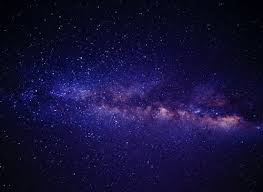
\includegraphics[scale=1]{Figures/universe}	
%	\caption{Sample picture of universe }
%	\label{fig:universe}
%\end{figure}


\section[Motivation]{\textbf{Motivation}}

\begin{itemize}
	\item Vedic mathematics helps in simplifying calculations.
	\item High-speed Area Efficient 3 operands Adder provides better speed and less area than carry save adder.\\
\end{itemize}

\section[Problem statement]{\textbf{Problem statement}}

To achieve better speed and area efficient 16x16 Vedic multiplier using High-speed Area Efficient three operands Adder and compare the same using 16x16 Vedic multiplier using Carry Save Adder.
\\
\\
\section[Objectives]{\textbf{Objectives}}
The objectives of the project are
\begin{enumerate}
\item To design a Verilog code and implement 16x16 Vedic multiplier using Carry Save Adder.
\item To design a Verilog code and implement 16x16 Vedic multiplier using High Speed Area Efficient 3 operands Adder.
\item Comparing delay and power consumption for both the adders.
\end{enumerate}

\section[Literature Review]{\textbf{Literature Review}}

To achieve optimal system performance while maintaining physical security, it is necessary to implement the cryptography algorithms on hardware [1] – [3]. Modular arithmetic such as modular exponentiation, modular multiplication and modular addition is frequently used for the arithmetic operations in various cryptography algorithms [4]. Therefore, the performance of the cryptography algorithm depends on the efficient implementation of the congruential modular arithmetic operation. The most efficient approach to implement the modular multiplication and exponentiation is the Montgomery algorithm [5] – [7] whose critical operation is based on three-operand binary addition [6] – [8]. The three-operand binary addition is also a primary arithmetic operation in the linear congruential generator (LCG) based pseudo-random bit generators (PRBG) such as coupled LCG (CLCG) [9], modified dual-CLCG (MDCLCG) [10] and coupled variable input LCG (CVLCG) [11]. Modified dual-CLCG (MDCLCG) is the most secure and highly random PRBG method among all the LCG-based and other existing PRBG methods. It is polynomial-time unpredictable and secure if n \_ 32-bits. Therefore, the security of the MDCLCG enhances with the increase of operand size. However, the area and critical path delay increases linearly since its hardware architecture consists of four three-operand modulo-2n adders, two comparators, four multiplexers area [10]. Hence, the performance of the MDCLCG can be improved by the efficient implementation of the three-operand adder. The three-operand binary addition can be carried out either by using two two-operand adders or one three-operand adder. Carry-save adder (CS3A) is the area-efficient and widely adopted technique to perform the three-operand binary addition in the modular arithmetic used in cryptography algorithms [5] – [8], [12] – [14] and PRBG methods [9] – [11]. However, the longer carry propagation delay in the ripple-carry stage of CS3A seriously influences the performance of the MDCLCG and other cryptography architectures on IoT based hardware devices. To shorten the critical path delay, a parallel prefixed two-operand adder such as Han-Carlson (HCA) can also be used for three-operand binary addition. It reduces the critical path delay in the order of O(log2 n) but increases the area in the order of O(n log2 n) [15]. Therefore, it is necessary to develop an efficient VLSI architecture to carry out the fast three-operand binary addition with minimum hardware resources. Hence, a new high-speed area-efficient adder technique is proposed using pre-compute bitwise addition followed by carry-prefix computation logic to perform the three-operand addition in this paper that consumes considerably less gate area while minimizing the propagation delay in comparison to the HCA-based three-operand adder (HC3A). 



\section[Brief Methodology of the project]{\textbf{Brief Methodology of the project}}
A 2x2 Vedic Multiplier is used to design 16x16 Vedic multiplier using carry save adder and high-speed area efficient (HSAE) adder. The fig.~\ref{fig:x1} shows the design of 2x2 Vedic Multiplier as shown below.
\begin{figure}[htb]
\centering
	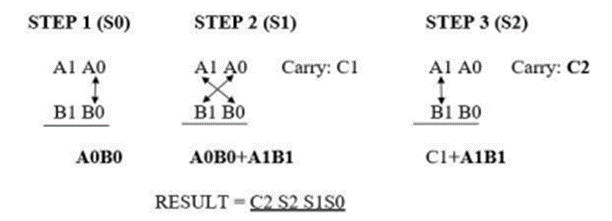
\includegraphics[scale=1]{Figures/x1}	
	\caption{2x2 Vedic Multiplier}
	\label{fig:x1}
\end{figure}
The design of 4x4 Vedic Multiplier using 2x2 Vedic Multiplier and CSA is shown below in fig.~\ref{fig:x2}
\begin{figure}[htb]
	\centering
	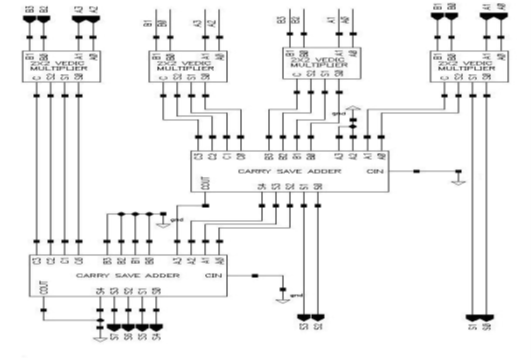
\includegraphics[scale=1]{Figures/x2}	
	\caption{4x4 Vedic Multiplier}
	\label{fig:x2}
\end{figure}
Similar to 4x4 Vedic Multiplier, the 8x8 and 16x16 Vedic Multipliers are designed using CSA and HSAE adder.
$S'\_{i}= a\_{i} \oplus b\_{i} \oplus c\_{i}$

\section[Organization of the report]{\textbf{Organization of the report}}

This report is organized as follows. Write the discussions in each chapter. A sample is as follows.
\begin{itemize}
\item Chapter 2 discusses the fundamentals of three-operand binary adder techniques.
\item Chapter 3 discusses the design of 16 x 16 Vedic multiplier.
\item Chapter 4 discusses the results and discussions.
\item Chapter 5 discusses the conclusion and future scope.
\end{itemize}

.

%Chapter 2
\chapter{Three-Operand Binary Adder Techniques}

The three-operands binary addition is one of the critical arithmetic operation in the congruential modular arithmetic architectures [5] – [8] and LCG-based PRBG methods such as CLCG [9], MDCLCG [10] and CVLCG [11]. It can be implemented either by using two stages of two-operands adders or one stage of three-operand adder.

\section{Three operands Carry Save Adder}
Carry-save adder (CSA) is the commonly used technique to perform the three-operand binary addition [9]–[14]. It computes the addition of three operands in two stages. The first stage is the array of full adders. Each full adder computes “carry” bit and “sum” bit concurrently from three binary input $ a_{i} $ , $ b_{i} $ and $ c_{i} $ . The second stage is the ripple-carry adder that computes the final n-bit size “sum” and one-bit size “carry-out” signals at the output of three-operand addition. The “carry-out” signal is propagated through the n number of full adders in the ripple-carry stage. Therefore, the delay increases linearly with the increase of bit length. The architecture of the three-operand carry-save adder is shown in Fig.~\ref{fig:x3} and the critical path delay is highlighted with a dashed line. It shows that the critical path delay depends on the carry propagation delay of ripple carry stage and is evaluated as follows,
\begin{equation}
 T_{CS3A} = (n+1)T_{FA} = 3T_{X} + 2_{n}T_{G}
 \label{eq1} 
\end{equation}
Similarly, the total area is evaluated as follows,
\begin{equation}
A_{CS3A} = 2nA_{FA} = 4nA_{X} + 6nA_{G}
	\label{eq2}
\end{equation}
Here, $ A_{G} $ and $ T_{G} $ indicate the area and propagation delay of basic 2-input gate (AND/OR/NAND/NOR) respectively. $ A_{X} $ and $ T_{X} $ indicate the area and propagation delay of 2-input XOR gate respectively. The major drawback of the CS3A is the larger critical path delay which increases with an increase of bit length. This critical propagation path delay influences the overall latency of the congruential modular arithmetic based cryptography and PRBG architectures, where three-operand adder is the primary component.
\begin{figure}[htb]
	\centering
	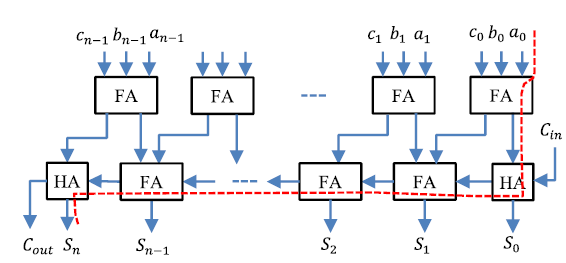
\includegraphics[width=0.80\columnwidth]{Figures/x3}	
	\caption{Three-operands carry-save adder (CS3A)}
	\label{fig:x3}
\end{figure}


\section{High-Speed Area Efficient Three Operands Adder}
This section presents a new adder technique and its VLSI architecture to perform the three-operand addition in modular arithmetic. The  adder technique is a parallel prefix adder.
\subsection{Overview of HSAE Adder}
The HSAE adder has four-stage structures instead three-stage structures in prefix adder to compute the addition of three binary input operands such as bit-addition logic, base logic, PG (propagate and generate) logic and sum logic. The logical expression of all these four stages is defined as follows,
\begin{figure}[htb]
	\centering
	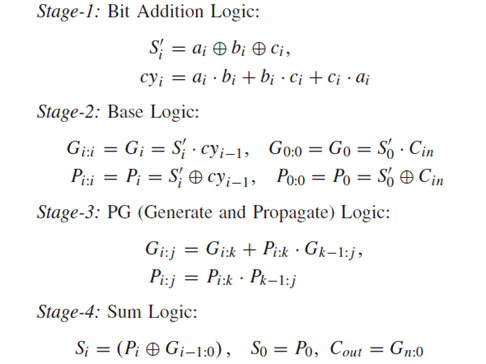
\includegraphics[width=0.80\columnwidth]{Figures/x4}	
%	\caption{Three-operands carry-save adder (CS3A)}
	\label{fig:x4}
\end{figure}
The proposed VLSI architecture of the three-operand binary adder and its internal structure is shown in Fig.~\ref{fig:x5}. The new adder technique performs the addition of three n-bit binary inputs in four different stages. In the first stage (bit-addition logic), the bitwise addition of three n-bit binary input operands is performed with the array of full adders, and each full adder computes “sum ($ S'_{i} $)” and “carry ($ cy_{i} $)” signals as highlighted in Fig.~\ref{fig:x5} (a). The logical expressions for computing sum ($ S'_{i} $) and carry ($ cy_{i} $ ) signals are defined in Stage-1, and the logical diagram of the bit-addition logic is shown in Fig.~\ref*{fig:x5} (b). \par 
In the first stage, the output signal “sum ($ S'_{i} $)” bit of current full adder and the output signal “carry” bit of its right-adjacent full adder are used together to compute the generate ($ G_{i} $) and propagate ($ P_{i} $) signals in the second stage (base logic). The computation of $ G_{i} $ and $ P_{i} $ signals are represented by the “squared saltire-cell” as shown in Fig.~\ref{fig:x5} (a) and there is n+1 number of saltire-cells in the base logic stage. The logic diagram of the saltire-cell is shown in Fig.~\ref{fig:x5} (b), and it is realized by the following logical expression,
\begin{equation}
G_{i:i} = G_{i} = S'_{i} \cdot cy_{i−1}
	\label{eq3}
\end{equation}
\begin{equation}
P_{i:i} = P_{i} = S'_{i} \cdot cy_{i−1}
	\label{eq4}
\end{equation}
The external carry-input signal ($ C_{in} $) is also taken into consideration for three-operand addition in the proposed adder technique. This additional carry-input signal ($ C_{in} $) is taken as input to base logic while computing the $ G_{0}(S'_{0} \cdot C_{in}) $ in the first saltire-cell of the base logic.
\begin{figure}[htb]
	\centering
	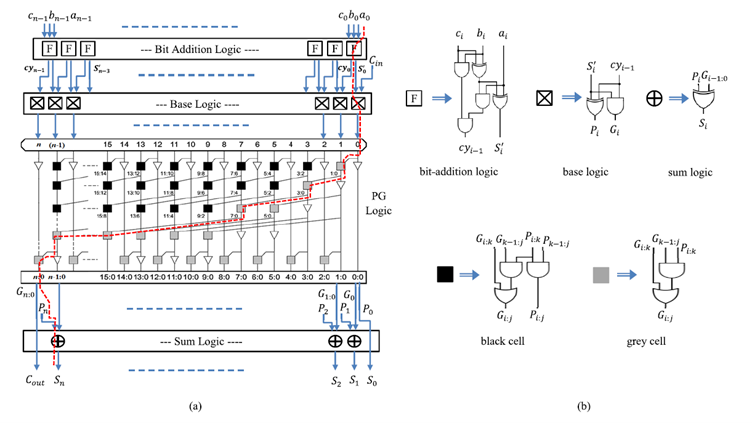
\includegraphics[width=0.80\columnwidth]{Figures/x5}	
	\caption{High Speed Area Efficient Adder}
	\label{fig:x5}
\end{figure}
The third stage is the carry computation stage called “generate and propagate logic” (PG) to pre-compute the carry bit and is the combination of black and grey cell logics. The logical diagram of black and grey cell is shown in Fig.~\ref{fig:x5} (b) that computes the carry generate $ G_{i:j} $ and propagate $ P_{i:j} $ signals with the following logical expression,
\begin{equation}
G_{i:j} = G_{i:k} + P_{i:k} \cdot G_{k−1:j}
	\label{eq5}
\end{equation}
\begin{equation}
P_{i:j} = P_{i:k} \cdot P_{k−1:j}
	\label{eq6}
\end{equation}
The number of prefix computation stages for the proposed adder is $(\log_{2}n + 1)$ , and therefore, the critical path delay of the proposed adder is mainly influenced by this carry propagate chain. \par
The final stage is represented as sum logic in which the “sum ($ S_{i} $)” bits are computed from the carry generate $ G_{i:j} $ and carry propagate $ P_{i} $ bits using the logical expression, $ S_{i} = (P_{i} \oplus G_{i−1:0}) $. The carryout signal ($ C_{out} $) is directly obtained from the carry generate bit $ G_{n:0} $.










%Chapter 3
\chapter{Design Of 16x16 Vedic Multiplier}

\indent\indent The Verilog code and the testbench are written for a 16x16 Vedic multiplier using a carry-save adder and high-speed area efficient adder.


\section{Verilog Code and Testbench for 16x16 Vedic Multiplier}
Figure ~\ref{fig:x1} illustrates the steps to multiply two 2-bit numbers. Converting the above figure to a hardware equivalent we have 3 and gates that will act as 2-bit multipliers and two half adders to add the products to get the final product. Here is the hardware detail of the multiplier.
\begin{figure}[htb]
	\centering
	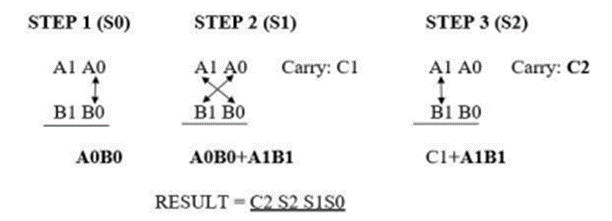
\includegraphics[width=0.80\columnwidth]{Figures/x1}	
	\caption{Steps to Multiply 2x2 Vedic Multiplier}
	\label{fig:x1}
\end{figure}
Where "a" and "b" are two numbers to be multiplied and "q" is the product. With this design we are now ready to code this in verilog easily using and gates and HA (half adders). To make the design more modular we try to write code for HA first and then instantiate it to have the final product. \\
\begin{figure}[htb]
	\centering
	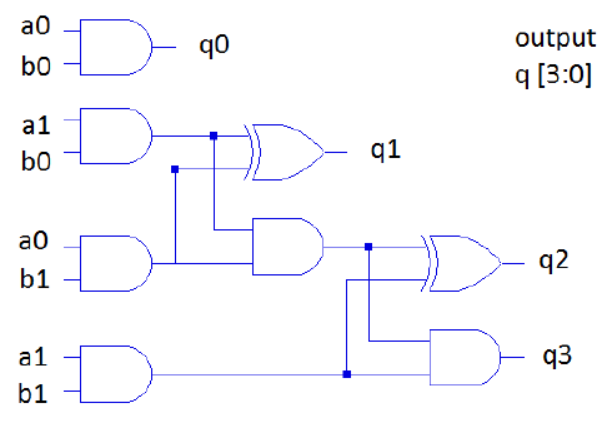
\includegraphics[width=0.5\columnwidth]{Figures/x6}	
	\caption{Design of 2x2 Vedic Multiplier}
	\label{fig:x6}
\end{figure}
The Verilog code for 2x2 Vedic Multiplier is \\
`timescale 1ns / 1ps\\
//////////////////////////////////////////////////////////////////////////////////\\
// Company: \\
// Engineer: \\
// \\
// Create Date:    12:34:18 08/01/2013 \\
// Design Name: \\
// Module Name:    vedic\_2\_x\_2 \\
// Project Name: \\
// Target Devices: \\
// Tool versions: \\
// Description: \\
//
// Dependencies: \\
//
// Revision: \\
// Revision 0.01 - File Created \\
// Additional Comments: \\
//\\
//////////////////////////////////////////////////////////////////////////////////\\
module vedic\_2\_x\_2(\\
a,\\
b,\\
c\\
    );\\
input [1:0]a;\\
input [1:0]b;\\
output [3:0]c;\\
wire [3:0]c;\\
wire [3:0]temp;\\
//stage 1\\
// four multiplication operation of bits according to vedic logic done using and gates \\
assign c[0]=a[0]\&b[0]; \\
assign temp[0]=a[1]\&b[0];\\
assign temp[1]=a[0]\&b[1];\\
assign temp[2]=a[1]\&b[1];\\
//stage two \\
// using two half adders \\
ha z1(temp[0],temp[1],c[1],temp[3]);\\
ha z2(temp[2],temp[3],c[2],c[3]);\\
endmodule\\
\\
The Verilog code for 4x4 Vedic Multiplier is\\
`timescale 1ns / 1ps\\
//////////////////////////////////////////////////////////////////////////////////\\
// Company: \\
// Engineer: \\
// \\
// Create Date:    14:30:08 08/01/2013 \\
// Design Name: \\
// Module Name:    vedic\_4\_x\_4 \\
// Project Name: \\
// Target Devices: \\
// Tool versions: \\
// Description: \\
//\\
// Dependencies: \\
//\\
// Revision: \\
// Revision 0$ \cdot $01 - File Created\\
// Additional Comments: \\
//\\
//////////////////////////////////////////////////////////////////////////////////\\
module vedic\_4\_x\_4(\\
a,b,c\\
    );\\
input [3:0]a;\\
input [3:0]b;\\
output [7:0]c;\\
\\
wire [3:0]q0;	\\
wire [3:0]q1;	\\
wire [3:0]q2;\\
wire [3:0]q3;	\\
wire [7:0]c;\\
wire [3:0]temp1;\\
wire [5:0]temp2;\\
wire [5:0]temp3;\\
wire [5:0]temp4;\\
wire [3:0]q4;\\
wire [5:0]q5;\\
wire [5:0]q6;\\
// using 4 2x2 multipliers\\
vedic\_2\_x\_2 z1(a[1:0],b[1:0],q0[3:0]);\\
vedic\_2\_x\_2 z2(a[3:2],b[1:0],q1[3:0]);\\
vedic\_2\_x\_2 z3(a[1:0],b[3:2],q2[3:0]);\\
vedic\_2\_x\_2 z4(a[3:2],b[3:2],q3[3:0]);\\
// stage 1 adders \\
assign temp1 ={2'b0,q0[3:2]};\\
add\_4\_bit z5(q1[3:0],temp1,q4);\\
assign temp2 ={2'b0,q2[3:0]};\\
assign temp3 ={q3[3:0],2'b0};\\
add\_6\_bit z6(temp2,temp3,q5);\\
assign temp4={2'b0,q4[3:0]};\\
// stage 2 adder \\
add\_6\_bit z7(temp4,q5,q6);\\
// fnal output assignment \\
assign c[1:0]=q0[1:0];\\
assign c[7:2]=q6[5:0];\\
\\
endmodule\\
\\
The Verilog code for 8x8 Vedic Multiplier is\\
\\
`timescale 1ns / 1ps \\
//////////////////////////////////////////////////////////////////////////////////\\
// Company: \\
// Engineer: \\
// \\
// Create Date:    15:22:39 08/01/2013 \\
// Design Name: \\
// Module Name:    vedic\_8X8 \\
// Project Name: \\
// Target Devices: \\
// Tool versions: \\
// Description: \\
//\\
// Dependencies: \\
//\\
// Revision: \\
// Revision 0.01 - File Created\\
// Additional Comments: \\
//\\
//////////////////////////////////////////////////////////////////////////////////\\
module vedic\_8X8(a,b,c\\
    );\\
   \\
input [7:0]a;\\
input [7:0]b;\\
output [15:0]c;\\
\\
wire [15:0]q0;	\\
wire [15:0]q1;	\\
wire [15:0]q2;\\
wire [15:0]q3;	\\
wire [15:0]c;\\
wire [7:0]temp1;\\
wire [11:0]temp2;\\
wire [11:0]temp3;\\
wire [11:0]temp4;\\
wire [7:0]q4;\\
wire [11:0]q5;\\
wire [11:0]q6;\\
// using 4 4x4 multipliers\\
vedic\_4\_x\_4 z1(a[3:0],b[3:0],q0[15:0]);\\
vedic\_4\_x\_4 z2(a[7:4],b[3:0],q1[15:0]);\\
vedic\_4\_x\_4 z3(a[3:0],b[7:4],q2[15:0]);\\
vedic\_4\_x\_4 z4(a[7:4],b[7:4],q3[15:0]);\\
\\
// stage 1 adders \\
assign temp1 ={4'b0,q0[7:4]};\\
add\_8\_bit z5(q1[7:0],temp1,q4);\\
assign temp2 ={4'b0,q2[7:0]};\\
assign temp3 ={q3[7:0],4'b0};\\
add\_12\_bit z6(temp2,temp3,q5);\\
assign temp4={4'b0,q4[7:0]};\\
// stage 2 adder\\
add\_12\_bit z7(temp4,q5,q6);\\
// fnal output assignment \\
assign c[3:0]=q0[3:0];\\
assign c[15:4]=q6[11:0];\\
\\
endmodule\\
\\
The Verilog code for 16x16 Vedic Multiplier is\\
\\
`timescale 1ns / 1ps\
//////////////////////////////////////////////////////////////////////////////////\\
// Company: \\
// Engineer: \\
// \\
// Create Date:    15:45:52 08/01/2013 \\
// Design Name: \\
// Module Name:    vedic\_16x16 \\
// Project Name: \\
// Target Devices: \\
// Tool versions: \\
// Description: \\
//\\
// Dependencies: \\
//\\
// Revision: \\
// Revision 0.01 - File Created\\
// Additional Comments: \\
//\\
//////////////////////////////////////////////////////////////////////////////////\\
module vedic\_16x16(a,b,c\\
    );\\
input [15:0]a;\\
input [15:0]b;\\
output [31:0]c;\\
\\
wire [15:0]q0;	\\
wire [15:0]q1;	\\
wire [15:0]q2;\\
wire [15:0]q3;	\\
wire [31:0]c;\\
wire [15:0]temp1;\\
wire [23:0]temp2;\\
wire [23:0]temp3;\\
wire [23:0]temp4;\\
wire [15:0]q4;\\
wire [23:0]q5;\\
wire [23:0]q6;\\
// using 4 8x8 multipliers\\
vedic\_8X8 z1(a[7:0],b[7:0],q0[15:0]);\\
vedic\_8X8 z2(a[15:8],b[7:0],q1[15:0]);\\
vedic\_8X8 z3(a[7:0],b[15:8],q2[15:0]);\\
vedic\_8X8 z4(a[15:8],b[15:8],q3[15:0]);\\
\\
// stage 1 adders \\
assign temp1 ={8'b0,q0[15:8]};\\
add\_16\_bit z5(q1[15:0],temp1,q4);\\
assign temp2 ={8'b0,q2[15:0]};\\
assign temp3 ={q3[15:0],8'b0};\\
add\_24\_bit z6(temp2,temp3,q5);\\
assign temp4={8'b0,q4[15:0]};\\
\\
//stage 2 adder\\
add\_24\_bit z7(temp4,q5,q6);\\
// final output assignment \\
assign c[7:0]=q0[7:0];\\
assign c[31:8]=q6[23:0];\\
\\
endmodule\\
\\
The Verilog Tesbench code for 16x16 Vedic Multiplier is\\
\\
`timescale 1ns / 1ps\\
\\
////////////////////////////////////////////////////////////////////////////////\\
// Company: \\
// Engineer:\\
//\\
// Create Date:   16:15:22 08/01/2013\\
// Design Name:   vedic\_16x16\\
// Module Name:   D:/lfsr/test\_vedic\_16 $ \cdot $ v\\
// Project Name:  lfsr\\
// Target Device:  \\
// Tool versions:  \\
// Description: \\
//\\
// Verilog Test Fixture created by ISE for module:\\ vedic\_16x16\\
//\\
// Dependencies:\\
// \\
// Revision:\\
// Revision 0$ \cdot $01 - File Created\\
// Additional Comments:\\
// \\
////////////////////////////////////////////////////////////////////////////////\\
\\
module test\_vedic\_16;\\
\\
	// Inputs\\
	reg [15:0] a;\\
	reg [15:0] b;\\
\\
	// Outputs\\
	wire [31:0] c;\\
\\
	// Instantiate the Unit Under Test (UUT)\\
	vedic\_16x16 uut (\\
		$ \cdot $a(a), \\
		$ \cdot $b(b), \\
		$ \cdot $c(c)\\
	);\\
\\
	initial begin\\
		// Initialize Inputs\\
		a = 0;\\
		b = 0;\\
		\# 100;\\
		\\
		a = 16'd12;\\
		b = 16'd12;\\
		\# 100;\\
		\\
		a = 16'd15;\\
		b = 16'd13;\\
		\# 100;\\
		\\
		a = 16'd24;\\
		b = 16'd2;\\
		\# 100;\\
		\\
		a = 16'd200;\\
		b = 16'd21;\\
		\# 100;\\
		\\
		a = 16'd36;\\
		b = 16'd48;\\
		\# 100;\\
        \\
		\\
\\
	end\\
      \\
endmodule\\
\\







%%Chapter 4
%\chapter{Implementation of Pipelined Analog to Digital converter}

\indent\indent From Chapter 2 onwards, every chapter should start with an introduction paragraph. This paragraph should brief about the flow of the chapter. This introduction can be limited within 4 to 5 sentences. The chapter heading should be appropriately modified (a sample heading is shown for this chapter).But don't start the introduction paragraph in the chapters 2 to end with "This chapter deals with....". Instead you should bring in the highlights of the chapter in the introduction paragraph. 

\section{Contents of this chapter}
This chapter should elaborate the following in detail.
\begin{enumerate}
\item Implementation details for hardware based projects
\item Top level Design for software based projects
\end{enumerate}

You can add sections and sub sections to elaborate your project work done.

\vspace{0.75cm}

 \textbf{The chapters should not end with figures, instead bring the paragraph explaining about the figure at the end followed by a summary paragraph.}

After elaborating the various sections of the chapter (From Chapter 2 onwards), a summary paragraph should be written discussing the highlights of that particular chapter. This summary paragraph should not be numbered separately. This paragraph should connect the present chapter to the next chapter. 



%Chapter 5
\chapter{Results \& Discussions}
\indent\indent This chapter provide details related to results of the design implementation. The results are divided as simulation result of 16 x 16 Vedic Multiplier using carry save adder and result of 16 x 16 Vedic Multiplier using high-speed area efficient adder.


\section{Simulation Result}
The simulation analysis of the 16 x 16 Vedic Multiplier using carry save adder and of 16 x 16 Vedic Multiplier using high-speed area efficient adder is carried out using Xilinx ISE Software. The simulation result is shown in Fig. \ref{fig:x7}.\\
\begin{figure}[htb]
	\centering
	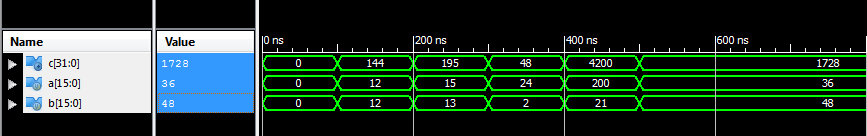
\includegraphics[width=0.9\columnwidth]{Figures/x7}	
	\caption{Simulation Result of 16 x 16 Vedic Multiplier}
	\label{fig:x7}
\end{figure}
Here A \& B are the input 16-bit data and C is the 32 bit multiplier output. One can easily observe that the output for 16 x 16 Vedic Multiplier using carry save adder and 16 x 16 Vedic Multiplier using high-speed area efficient adder has been obtained successfully. The multiplication of 21 \& 200 yields 4200 and multiplication of 13 \& 15 yields 195, simlarly the other multiplication input combinations can be observed and the results are true with no errors.
\begin{table}[htb]
\fontsize{10}{12}\selectfont
\caption{Comparision of Critical Path Delay and Total Power}
\label{tab:tab1}
\centering
\begin{tabular}{@{}|c|c|c|c|@{}}
\toprule
\textbf{SL NO} & \textbf{\begin{tabular}[c]{@{}c@{}}16x16 Vedic Multiplier\\ using\end{tabular}} & \textbf{\begin{tabular}[c]{@{}c@{}}Critical Path\\ Delay(ns)\end{tabular}} & \textbf{\begin{tabular}[c]{@{}c@{}}Total Power \\ (µW)\end{tabular}} \\ \midrule
1              & \textbf{CSA}                                                                    & 0.882                                                                 & 70                                                                   \\ \midrule
2              & \textbf{HSAE Adder}                                                             & 0.824                                                                 & 55                                                                   \\ \bottomrule
\end{tabular}
\end{table}
From the table \ref{tab:tab1} we can observe the results that the 16x16 Vedic Multiplier using High-speed-area-efficient adder is having the total power and critical path delay of 55µW and 824ps respectively which is much better as compared to 16x16 Vedic Multiplier using CSA.






%Chapter 6
\chapter{Conclusion and Future Scope}

\section{Conclusion}
Multiplication is a resource hungry operation and is a major computational need in complex circuits. Through literature survey, it was found that As multipliers play a critical role in any digital design. It is necessary to implement faster multipliers occupying lesser area and consuming less power. Multiplication operation can be done using Array multiplier, redundant binary structures and tree structures but they have problem of larger delay. Vedic Multipliers are faster compared to traditional Array multiplier, Wallace tree multiplier etc.\\
The 16x16 Vedic Multiplier using High-speed-area-efficient adder is having the power consumption and total delay of 55µW and 824ps respectively which is much better as compared to 16x16 Vedic Multiplier using CSA.


\section{Future Scope}
Further work can be taken up to increase bit-length and improve accuracy. Also, this modified Vedic Multiplier can be tested on different dataset or can be explored for different application.




%% Uncomment the following 2 commands to add Appendix chapters
%\appendix
%\chapter{Code}
\section{First Appendix}
You can use \texttt{tcblisting} for creating the code snippets. The following example illustrates how one can customize the \texttt{tcblisting} to achieve the \texttt{tcl} script. Similarly, one can use it for other programming language listing, including HDL.

\begin{tcblisting}{listing only,colback=gray!10!white, breakable, boxsep=0pt,top=1mm,bottom=1mm,left=1mm,right=1mm,
listing options={
language= tcl,
basicstyle=\small\ttfamily, 
otherkeywords={create_clock, set_clock_latency, set_input_delay, set_output_delay, set_load, set_max_fanout, set_fanout_load},
keywordstyle=\color{blue}, 
%keywordstyle=[2]{\color{red}},
commentstyle=\color{gray},
backgroundcolor=\color{gray!25},
%morekeywords=[2]{arg,pos},
%moredelim=[is][\color{violet}]{''}{''},
escapechar=!}}
# Since our design has a clock with name clk, 
## specify that name under [get_port ]
create_clock -period 40 -waveform {0 20} [get_ports clk]

# Setting a 'delay' on the clock:
set_clock_latency 0.3 clk

# Setting up constraints on your I/P and O/P pins
set_input_delay 2.0 -clock clk [all_inputs]!\tikz[remember picture]\node[](c1){};!
set_output_delay 1.65 -clock clk [all_outputs]!\tikz[remember picture]\node[](c2){};!

# Set realistic 'loads' on each output pin
set_load 0.1 [all_outputs]

# Set 'maximum' fanin and fan-out for the input and output pins 
set_max_fanout 1 [all_inputs]
set_fanout_load 8 [all_outputs]      
\end{tcblisting}%Appendix Chapter 1

\backmatter
\clearpage
\printbibliography%
% Please don't use \cite command in content/text, if you use \cite command then you need to do changes in \nocite{*} command accordingly 
\nocite{*}

\end{spacing}
\end{document}
